\chapter{Kravspecifikation}

For at definere hvad dette projekt handler om er det vigtigt at sætte rammer for hvad der helt præcist er tiltænkt. For at gøre dette er nedenstående use cases lavet for at gøre nogle af brugssituationerne med drink maskinen lidt klare.

\begin{figure}[H]
	\centering
	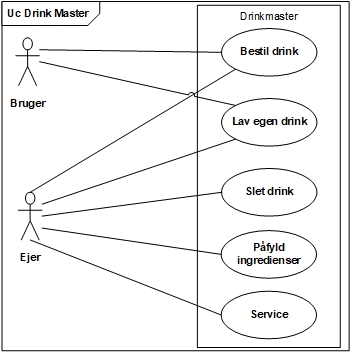
\includegraphics[scale=1.2]{Images/UC_diagram_JPEG.jpg}
	\caption{Aktør-Kontekst diagram for Drink Master}
	\label{fig:uc_actor_context}
\end{figure}
\FloatBarrier

\newpage
\section{Use cases}
\subsection{Use case beskrivelser}
\begin{itemize}
    \item UC1: \textbf{Bestil Drink} $-$ Det essentielle ved maskinen skal være at man kan bestille drinks, lige som man ville gøre ved en bartender, men hvor blandingen af drinken sker automatisk ud fra hvordan man selv har defineret drinken til at være.
    
    \item UC2: \textbf{Lav egen drink} $-$ Der er ikke nogle drinks i drink maskinen til at starte med, så der skal tilføjes nogle inden man kan bestille en drink. Når man opretter en drink skal der angives type væske om mængden af væsken. Man kan oprette så mange drinks man vil, og man kan oprette flere af de samme, med få nyancer. Fx 1 drink med 2 cl vodka og en anden med 4 cl vodka.
    
    %\item UC2: \textbf{Opret drink} $-$ Der er ikke nogle drinks i drink maskinen til at starte med, så der skal tilføjes nogle inden man kan bestille en drink. Når man opretter en drink skal der angives type væske om mængden af væsken. Man kan oprette så man drinks man vil, og man kan oprette flere af de samme, med få nyancer. Fx 1 drink med 2 cl vodka og en anden med 4 cl vodka.
    
    \item UC3: \textbf{Slet drink} $-$ Denne er tiltænkt for at ejer af maskinen skal kunne slette drinks efter de er oprettet. Dette er fordi man kan komme til at oprette en drink anderledes end den var tiltænkt, men også fordi det skal give ejer mulighed for at slette drinks der er tilføjet den aften maskinen blev brugt, som man nu ikke længere gider at have på listen længere. 
    
    \item UC4: \textbf{Påfyld ingredienser} $-$ Når der en flaske der er ved at være tom, skal den udskiftes. Denne use case er til dette scenarie. Det er dog implicit at der i forvejen er tilføjet en flaske og at man selv skal fjerne flasken. Maskinens system vil give besked om når der er 10 mL væske i flasken tilbage.
    
    %\item UC4: \textbf{Tilføj flaske} $-$ Lige som der ikke er nogle drinks tilføjet i maskinen til at starte med, så er der heller ikke nogle flasker tilføjet til maskinen. For at tilføje en flaske til maskinen, skal flasken både gøres fysisk og i selve programmet. Dvs. man først montere flasken på maskinen og derefter angiver man i programmet hvor man har sat flasken og hvad man har sat der.
    
    %\item UC5: \textbf{Fjern flaske} $-$ Når en flaske har under 10ml tilbage, signalerer maskinen at flasken snart er tom. Dette er for at man kan få et heads-up på hvornår der skal tilføjes en ny flaske.
    
    \item UC5: \textbf{Service} $-$ Når systemet har lavet X antal drinks, giver maskinen besked om at den trænger til at blive ckecket for væskerester og andet der evt. kan trigge en tiltrængt rengøring. Touchskærmen kan være fedtet, der hvor flaskerne står kan der være væskerester og andre ting kan være fedtede med sukkerindeholdige væsker.
\end{itemize}

\subsection{UC1: Bestil drink}
\begin{table}[H]
\begin{tabular}{|p{5cm}|p{9cm}|}
\hline
\rowcolor[HTML]{C0C0C0} 
\textbf{Navn:} & Bestil drink\\ \hline
\textbf{Mål:} & Bruger modtager den bestilte drink\\ \hline
\rowcolor[HTML]{C0C0C0} 
\textbf{Initiering:} & Bruger går over til touchskærmen som tænder\\ \hline
\textbf{Aktører:} & Bruger/ejer\\ \hline
\rowcolor[HTML]{C0C0C0} 
\textbf{Antal samtidige forekomster:} & 1\\ \hline
\textbf{Prækondition:} & Drinkmaster er funktionsdygtig og brugeren har placeret et glas i systemet. \\ \hline
\rowcolor[HTML]{C0C0C0} 
\textbf{Postkondition:} & Kunden tager den bestilte drink\\ \hline
\begin{tabular}[c]{@{}l@{}} \textbf{Hovedscenarie:} \\ \\ \\ \\ \\ \\ \\ \\ \\ \\ \end{tabular}& \begin{tabular}[c]{@{}l@{}}
1. Systemets touchscreen viser en liste af mulige drinks.\\
2. Brugeren vælger drink på touchscreen.\\
3. Systemet modtager brugerens valg.\\
4. Systemet undersøger om der er tilstrækkelige mængder \\ \hspace*{4mm}af ingredienser til at lave drinken. \\\hspace*{4mm}\textit{[EXT 1: Ikke tilstrækkelige mængder af ingredienser]}\\
5. Systemet doserer drinkens ingredienser i glasset. \\
6. Systemet viser beskeden ”Valgte drink er klar – tag \\ \hspace*{4mm}din drink” på touchscreen.\\
7. Brugeren tager glasset med drinken og UC afsluttes. \\
\end{tabular}\\ \hline
\rowcolor[HTML]{C0C0C0} 
\textbf{Udvidelser/undtagelser:} & \begin{tabular}[c]{@{}l@{}}
\textit{[EXT 1: Ikke tilstrækkelige mængder af ingredienser]}\\ 
1. UC 4 initieres.\\
2. UC 4 afsluttes og use casen returnerer til punkt 5. \\
\end{tabular}\\ \hline
\end{tabular}
\end{table}

\subsection{UC2: Lav egen drink}
\begin{table}[H]
\begin{tabular}{|p{5cm}|p{9cm}|}
\hline
\rowcolor[HTML]{C0C0C0} 
\textbf{Navn:} & Lav egen drink\\ \hline
\textbf{Mål:} & At brugeren tilføjer en drink til databasen\\ \hline
\rowcolor[HTML]{C0C0C0} 
\textbf{Initiering:} & Bruger går over til touchskærmen som tænder\\ \hline
\textbf{Aktører:} & Bruger/ejer\\ \hline
\rowcolor[HTML]{C0C0C0} 
\textbf{Antal samtidige forekomster:} & 1\\ \hline
\textbf{Prækondition:} & Maskinen er er tændt og aktiveret. \\ \hline
\rowcolor[HTML]{C0C0C0} 
\textbf{Postkondition:} & Der er oprettet en brugerdefineret drink i databasen og maskinen er klar til næste operation\\ \hline
\begin{tabular}[c]{@{}l@{}} \textbf{Hovedscenarie:} \\ \\ \\ \\ \\ \\ \\ \\ \\ \\ \\ \\ \\\end{tabular}& \begin{tabular}[c]{@{}l@{}}
1. Systemet registrerer at bruger er indenfor 75 cm og \\\hspace*{4mm} touchskærm tænder.\\
2. Bruger vælger "Opret drink" på touchskærmen.\\
3. Bruger bedes indtaste et navn på den ønskede drink.\\
4. Bruger indtaster navn på den ønskede drink og \\ \hspace*{4mm}trykker "OK". \\
5. En liste over tilgængelige væsker vises. \\
6. Bruger vælger en ønsket væske og angiver i boksen ud\\ \hspace*{4mm}for den valgte væske, den mængde der skal bruges.\\
\hspace*{4mm}\textit{[EXT1: Der skal tilføjes flere ingredienser til den}\\ \hspace*{4mm}\textit{ønskede drink].}\\%\hspace*{4mm}
7. Bruger trykker "Tilføj drink". \\\hspace*{4mm}\textit{[EXT2: Bruger trykker på annuller]}\\
\end{tabular}\\ \hline
\rowcolor[HTML]{C0C0C0} 
\textbf{Udvidelser/undtagelser:} & \begin{tabular}[c]{@{}l@{}}
\textit{[EXT1: Der skal tilføjes flere ingredienser til den}\\\hspace*{12mm} \textit{ønskede drink]}\\ 
1. Går til punkt 6 igen.\\
\textit{[EXT2: Ikke tilstrækkelige mængder af ingredienser]}\\ 
1. Går tilbage til startskærmen.\\
2. Der blev ikke oprettet en ny drink. \\
\end{tabular}\\ \hline
\end{tabular}
\end{table}

\subsection{UC3: Slet drink}

\begin{table}[H]
\begin{tabular}{|p{5cm}|p{9cm}|}
\hline
\rowcolor[HTML]{C0C0C0} 
\textbf{Navn:} & Slet drink\\ \hline
\textbf{Mål:} & At ejeren har slettet en drink i listen over drinks\\ \hline
\rowcolor[HTML]{C0C0C0} 
\textbf{Initiering:} & Ejer vælger "Fjern drik"\\ \hline
\textbf{Aktører:} & Ejer\\ \hline
\rowcolor[HTML]{C0C0C0} 
\textbf{Antal samtidige forekomster:} & 1\\ \hline
\textbf{Prækondition:} & Ejer  har  tilstrækkelige  rettigheder  til  at  kunne  slette  en drink fra databasen. Touchskærmen er tændt. \\ \hline
\rowcolor[HTML]{C0C0C0} 
\textbf{Postkondition:} & En drink er blevet slettet fra drinkdatabasen og dette er også opdateret på listen til maskinen.\\ \hline
\begin{tabular}[c]{@{}l@{}} \textbf{Hovedscenarie:} \\ \\ \\ \\ \\ \\ \\ \\\end{tabular}& \begin{tabular}[c]{@{}l@{}}
1. Ejer vælger "Slet drink"på touchskærmen.\\
2. En liste over nuværende drinks vises til brugeren.\\
3. Ejeren trykker på den drink som ønskes slettet.\\
4.Touchskærmen viser en besked:” Vil du slette den\\
\hspace*{4mm}valgtedrink?\\
5. Ejer trykker på "Ja". \\
\hspace*{4mm}\textit{[EXT 1: Ejer trykker "nej"]}\\
6. Touch skærm viser beskeden ”Drink slettet”.
\end{tabular}\\ \hline
\rowcolor[HTML]{C0C0C0} 
\textbf{Udvidelser/undtagelser:} & \begin{tabular}[c]{@{}l@{}}
\textit{[EXT 1: Ejer trykker "nej"]}\\ 
1. Systemet går tilbage til siden med listen over drinks.\\
2. Der blev ikke slettet en drink. \\
\end{tabular}\\ \hline
\end{tabular}
\end{table}


\subsection{UC4: Påfyld ingredienser}

\begin{table}[H]
\begin{tabular}{|p{5cm}|p{9cm}|}
\hline
\rowcolor[HTML]{C0C0C0} 
\textbf{Navn:} & Påfyld ingredienser\\ \hline
\textbf{Mål:} & At fylde ingredienser i systemet\\ \hline
\rowcolor[HTML]{C0C0C0} 
\textbf{Initiering:} & Ejer går hen til systemet\\ \hline
\textbf{Aktører:} & Ejer\\ \hline
\rowcolor[HTML]{C0C0C0} 
\textbf{Antal samtidige forekomster:} & 1\\ \hline
\textbf{Prækondition:} & At den flaske som skal udskiftes har <10cl tilbage.\\ \hline
\rowcolor[HTML]{C0C0C0} 
\textbf{Postkondition:} & Der er blevet lagt en ny, fuld flaske i systemet og den er klar til at hælde drinks op.\\ \hline
\begin{tabular}[c]{@{}l@{}} \textbf{Hovedscenarie:} \\ \\ \\ \\ \\ \\ \\ \\ \\ \\\end{tabular}& \begin{tabular}[c]{@{}l@{}}
1. Bruger/ejer vælger at lave en drink. \\
2. Touchskærmen giver besked om at en eller flere\\ \hspace*{4mm}ingredienser skal genopfyldes..\\
3. Ejer vælger "Udskift ingrediens".\\
4. Ejer afmonterer den valgte flaske og påsætter den nye\\ \hspace*{4mm}flaske. \\
5. Ejer trykker herefter på touch displayet "Ingrediens\\ \hspace*{4mm}udskiftet".\\
6. Systemet laver den bestilte drink.\\ 
7. Use case afsluttet.
\end{tabular}\\ \hline
\rowcolor[HTML]{C0C0C0} 
\textbf{Udvidelser/undtagelser:} & \\ \hline

\end{tabular}
\end{table}

\iffalse %Udkommentering start
\subsection{UC4: Tilføj flaske}

\begin{table}[H]
\begin{tabular}{|p{5cm}|p{9cm}|}
\hline
\rowcolor[HTML]{C0C0C0} 
\textbf{Navn:} & Tilføj flaske\\ \hline
\textbf{Mål:} & At en flaske er blevet tilføjet maksinen fysisk og at flasken er registreret i maskinens system.\\ \hline
\rowcolor[HTML]{C0C0C0} 
\textbf{Initiering:} & Bruger vil gerne tilføje en ny flaske til maskinen\\ \hline
\textbf{Aktører:} & Bruger\\ \hline
\rowcolor[HTML]{C0C0C0} 
\textbf{Antal samtidige forekomster:} & 1\\ \hline
\textbf{Prækondition:} & Der er plads til at blive tilføjet mindst én flaske i maskinen. Flaskeholderne er indexeret og markeret med tal\\ \hline
\rowcolor[HTML]{C0C0C0} 
\textbf{Postkondition:} & Der er fysisk blevet tilføjet en flaske og flasken er også registreret i maskinens system.\\ \hline
\begin{tabular}[c]{@{}l@{}} \textbf{Hovedscenarie:} \\ \\ \\ \\ \\ \\ \\ \\\end{tabular}& \begin{tabular}[c]{@{}l@{}}
1. Bruger sætter en flaske i en af flaskeholderne.\\
2. Bruger trykker på "Tilføj flaske" på touchskærmen.\\
3. På touchskærmen skal bruger nu angive hvilken position \\ \hspace*{4mm}flasken er sat på og hvad der er sat.\\
4.I systemet vælger bruger den samme position som bruger\\
\hspace*{4mm}fysisk har sat flasken på.\\
5. I systemet angiver bruger hvilken type flaskens\\  \hspace*{4mm}indhold er.\\
6. Bruger trykker "Bekræft tilføjelse".
\\\hspace*{4mm}\textit{[EXT 1: Bruger trykker på annuller]}\\
\end{tabular}\\ \hline
\rowcolor[HTML]{C0C0C0} 
\textbf{Udvidelser/undtagelser:} & \begin{tabular}[c]{@{}l@{}}
\textit{[EXT 1: Bruger trykker på "annuller"]}\\ 
1. Systemet går tilbage til hovedmenuen.\\
2. Der er endnu ikke tilføjet en flaske til systemet. \\
\end{tabular}\\ \hline
\end{tabular}
\end{table}

\subsection{UC5: Fjern flaske}
\begin{table}[H]
\begin{tabular}{|p{5cm}|p{9cm}|}
\hline
\rowcolor[HTML]{C0C0C0} 
\textbf{Navn:} & Fjern flaske\\ \hline
\textbf{Mål:} & At have fysisk fjernet en flaske fra maskinen og også fjernet den i systemet\\ \hline
\rowcolor[HTML]{C0C0C0} 
\textbf{Initiering:} & Bruger bestiller en drink.\\ \hline
\textbf{Aktører:} & Bruger\\ \hline
\rowcolor[HTML]{C0C0C0} 
\textbf{Antal samtidige forekomster:} & 1\\ \hline
\textbf{Prækondition:} & Bruger vil gerne fjerne en flaske - måske fordi indholdet i en af flaskerne er 10 cl. eller under.\\ \hline
\rowcolor[HTML]{C0C0C0}
\textbf{Postkondition:} & Den ønskede flaske er fjernet og dette er registreret i systemet.\\ \hline
\begin{tabular}[c]{@{}l@{}} \textbf{Hovedscenarie:} \\ \\ \\ \\ \\ \\ \\ \\ \\ \\ \\ \\ \\ \\\end{tabular}& \begin{tabular}[c]{@{}l@{}}
1. Touchskærmen giver besked om at en eller flere \\\hspace*{4mm}flasker er ved at være tomme. \\
2. Bruger fjerner den flaske der er ved at være tom \\
3. Bruger vælger "Fjern flaske" på touckskærm. \\
4. Bruger præsenteres for flaskeplaceringer med flasker \\\hspace*{4mm} registreret på deres plads.\\
5. Bruger vælger den flaskeplacering som tilhøre den flaske\\
\hspace{1mm}han/hun lige har fjernet.\\
6. Systemet giver beskeden "Er du sikker på at du vil fjerne\\
\hspace*{4mm}denne flaske fra systemet?"\\
7. Bruger trykker "Ja". Hvis bruger trykker "Nej", kan \\ 
\hspace*{4mm} bruger vælge en anden flaske at fjerne\\
\hspace*{4mm} eller gå tilbage til hovedmenuen ved at trykke på\\
\hspace*{4mm}"Tilbage"\\
8. Systemet fjerner flasken fra systemet og returnerer til\\
\hspace*{4mm}hovedmenu\\
\end{tabular}\\ \hline
\rowcolor[HTML]{C0C0C0} 
\textbf{Udvidelser/undtagelser:} & Ingen \\ \hline
\end{tabular}
\end{table}

\fi %udkommentering slut

\subsection{UC5: Service}

\begin{table}[H]
\begin{tabular}{|p{5cm}|p{9cm}|} 
\hline
\rowcolor[HTML]{C0C0C0} 
\textbf{Navn:} & Service\\ \hline
\textbf{Mål:} & At drink maskinen er rent og fuld funktionalitet er nu garanteret.\\ \hline
\rowcolor[HTML]{C0C0C0} 
\textbf{Initiering:} & Systemet registrerer at X antal drinks er lavet.\\ \hline
\textbf{Aktører:} & Ejer\\ \hline
\rowcolor[HTML]{C0C0C0} 
\textbf{Antal samtidige forekomster:} & 1\\ \hline
\textbf{Prækondition:} & Systemet har lavet det maksimal tilladte antal drinks.\\ \hline
\rowcolor[HTML]{C0C0C0} 
\textbf{Postkondition:} & Der er udført service på drinksmaskinen\\ \hline
\begin{tabular}[c]{@{}l@{}} \textbf{Hovedscenarie:} \\ \\ \\ \\ \\ \\ \\ \\ \\ \\ \\\end{tabular}& \begin{tabular}[c]{@{}l@{}}
1. Systemet giver besked til Ejer om at den  \\\hspace*{4mm}trænger til at blive serviceret.\\
2. Ejer trykker ”ok”. \\
3. Touchskærmen returnerer til hovedmenu, og er fuld \\ funktionel. \\
4. Ejer trykker service. \\
5. Touchskærm går i servicemode. \\
6. Ejer servicerer maskinen. \\
7. Ejer trykker ”Afslut service”. \\
8. System returnerer til hovedmenuen. \\
9. Use case afsluttes. \\
\end{tabular}\\ \hline
\rowcolor[HTML]{C0C0C0} 
\textbf{Udvidelser/undtagelser:} & Ingen \\ \hline
\end{tabular} 
\end{table} 

\section{Test Use cases:}

\begin{itemize}
    \item TUC1: Registrer bruger
    \item TUC2: Vægt registrerer kop
    \item TUC3: Ændre flaskeposition
    \item TUC4: Doser væske
    \item TUC5: Registrer tom flaske
    \item TUC6: PSoC master fortæller RPi at drink er færdig
\end{itemize}

\subsection{TUC 1: Registrer bruger}
\begin{table}[H]
\begin{tabular}{|p{5cm}|p{9cm}|}
\hline
\rowcolor[HTML]{C0C0C0} 
\textbf{Navn:} & Registrer bruger\\ \hline
\textbf{Mål:} & Motionsensor registrerer bruger og tænder for touchscreen\\ \hline
\rowcolor[HTML]{C0C0C0} 
\textbf{Initiering:} & Bruger\\ \hline
\textbf{Aktører:} & Bruger\\ \hline
\rowcolor[HTML]{C0C0C0} 
\textbf{Antal samtidige forekomster:} & 1\\ \hline
\textbf{Prækondition:} & Touchscreen er slukket \\ \hline
\rowcolor[HTML]{C0C0C0} 
\textbf{Postkondition:} & Touchscreen er tændt og systemet er klar til at modtage bestilling.\\ \hline
\begin{tabular}[c]{@{}l@{}} \textbf{Hovedscenarie:} \\ \\ \\ \\\end{tabular}& \begin{tabular}[c]{@{}l@{}}
1. Bruger går hen til systemet. \\
2. Proximitysensor registrerer bruger. \\
3. Proximitysensor sender signal til RPi. \\
4. RPi tænder for touchscreen. \\
\end{tabular}\\ \hline
\rowcolor[HTML]{C0C0C0} 
\textbf{Udvidelser/undtagelser:} & Ingen\\ \hline
\end{tabular}
\end{table}

\subsection{TUC 2: Vægt registrerer kop}
\begin{table}[H]
\begin{tabular}{|p{5cm}|p{9cm}|}
\hline
\rowcolor[HTML]{C0C0C0} 
\textbf{Navn:} & Vægt registrerer kop\\ \hline
\textbf{Mål:} & Vægt registrere kop og enabler "bestil drink"\\ \hline
\rowcolor[HTML]{C0C0C0} 
\textbf{Initiering:} & Bruger\\ \hline
\textbf{Aktører:} & Bruger\\ \hline
\rowcolor[HTML]{C0C0C0} 
\textbf{Antal samtidige forekomster:} & 1\\ \hline
\textbf{Prækondition:} & Der står ikke en kop i forvejen og systemet er ikke i gang med at brygge en drink.\\ \hline
\rowcolor[HTML]{C0C0C0} 
\textbf{Postkondition:} & \begin{tabular}[c]{@{}l@{}}Knappen "bryg drink" på touchskærm er enabled\end{tabular} \\ \hline
\begin{tabular}[c]{@{}l@{}} \textbf{Hovedscenarie:} \\ \\ \\ \\ \\ \end{tabular} & \begin{tabular}[c]{@{}l@{}}
1. Bruger sætter sin kop til opfylding. \\
2. Vægtens load cell sender signaler til PSoC Slave. \\
4. PSoC Slave sender data til PSoC master. \\
5. PSoC Master sender data til RPi \\
6. RPi enabler "Bryg drink" på GUI \\
\end{tabular}\\ \hline
\rowcolor[HTML]{C0C0C0} 
\textbf{Udvidelser/undtagelser:} & ingen\\ \hline
\end{tabular}
\end{table}

\subsection{TUC 3: Ændre flaskeposition}
\begin{table}[H]
\begin{tabular}{|p{5cm}|p{9cm}|}
\hline
\rowcolor[HTML]{C0C0C0} 
\textbf{Navn:} & Ændre flaskeposition.\\ \hline
\textbf{Mål:} & Systemet drejer ønsket flaske frem til doseringspositionen\\ \hline
\rowcolor[HTML]{C0C0C0} 
\textbf{Initiering:} & Bruger\\ \hline
\textbf{Aktører:} & Bruger\\ \hline
\rowcolor[HTML]{C0C0C0} 
\textbf{Antal samtidige forekomster:} & 1\\ \hline
\textbf{Prækondition:} & Systemet er tændt og klar til brug. \\ \hline
\rowcolor[HTML]{C0C0C0} 
\textbf{Postkondition:} & Systemet har drejet den ønskede flaske frem til doseringspositionen.\\ \hline
\begin{tabular}[c]{@{}l@{}} \textbf{Hovedscenarie:} \\ \\ \\ \\ \\ \\ \\ \end{tabular}& \begin{tabular}[c]{@{}l@{}}
1. Bruger vælger ønsket flaske på touchscreen. \\
2. RPi sender signal til PSoC Master. \\
3. PSoC Master sender signal til PSoC Slave. \\
4. PSoC Slave tænder steppermotor. \\
5. Steppermotor drejer flaskebeholder rundt. \\
6. Steppermotor stopper når ønsket flaske er ved \\\hspace*{4mm}doseringsposition. \\
\end{tabular}\\ \hline
\rowcolor[HTML]{C0C0C0} 
\textbf{Udvidelser/undtagelser:} & Ingen\\ \hline
\end{tabular}
\end{table}

\subsection{TUC 4: Doser væske}
\begin{table}[H]
\begin{tabular}{|p{5cm}|p{9cm}|}
\hline
\rowcolor[HTML]{C0C0C0} 
\textbf{Navn:} & Doser væske\\ \hline
\textbf{Mål:} & Systemet doserer den ønskede mængde væske\\ \hline
\rowcolor[HTML]{C0C0C0} 
\textbf{Initiering:} & Bruger\\ \hline
\textbf{Aktører:} & Bruger\\ \hline
\rowcolor[HTML]{C0C0C0} 
\textbf{Antal samtidige forekomster:} & 1\\ \hline
\textbf{Prækondition:} & Systemet er tændt og klar til brug. \\ \hline
\rowcolor[HTML]{C0C0C0} 
\textbf{Postkondition:} & Systemet har doseret den rigtige mængde væske i glasset.\\ \hline
\begin{tabular}[c]{@{}l@{}} \textbf{Hovedscenarie:} \\ \\ \\ \\ \\ \\\end{tabular}& \begin{tabular}[c]{@{}l@{}}
1. Bruger vælger ønsket mængde væske på touchscreen. \\
2. RPi sender besked til PSoC Master. \\
3. PSoC Master sender signal til PSoC Slave. \\
4. PSoC Slave tænder for pumpen ved flasken der er ved\\ \hspace*{4mm}doseringspositionen.\\
5. Pumpen stopper når ønsket mængde væske er doseret. \\
\end{tabular}\\ \hline
\rowcolor[HTML]{C0C0C0} 
\textbf{Udvidelser/undtagelser:} & Ingen\\ \hline
\end{tabular}
\end{table}

\subsection{TUC 5: Registrer tom flaske}
\begin{table}[H]
\begin{tabular}{|p{5cm}|p{9cm}|}
\hline
\rowcolor[HTML]{C0C0C0} 
\textbf{Navn:} & Registrer tom flaske \\ \hline
\textbf{Mål:} & Systemet skal registrerer at en flaske indeholder mindre en 10 cl, og sende besked til touchscreen\\ \hline
\rowcolor[HTML]{C0C0C0} 
\textbf{Initiering:} & Bruger går hen til touchskærmen, og motion sensor registrerer bevægelse \\ \hline
\textbf{Aktører:} & Bruger\\ \hline
\rowcolor[HTML]{C0C0C0} 
\textbf{Antal samtidige forekomster:} & 1\\ \hline
\textbf{Prækondition:} & Drinkmaster mangler IKKE service og klar til brug. Den valgte flaske indeholder 70 cl \\ \hline
\rowcolor[HTML]{C0C0C0} 
\textbf{Postkondition:} & Systemet har registreret at en flaskes indhold er 10 cl eller mindre \\ \hline
\begin{tabular}[c]{@{}l@{}} \textbf{Hovedscenarie:} \\ \\ \\ \\\end{tabular}& \begin{tabular}[c]{@{}l@{}}
1. Bruger vælger at doserer 60 cl fra en flaske. \\
2. [Test Use case 4 Initieres med 60 cl] \\
4. Bruger vælger at doserer 5 cl fra samme flaske. \\
5. Rpi udskriver, at flasken er ved at være tom \\
\end{tabular}\\ \hline
\rowcolor[HTML]{C0C0C0} 
\textbf{Udvidelser/undtagelser:} & Ingen\\ \hline
\end{tabular}
\end{table}


\subsection{TUC 6: PSoC master fortæller RPi at drink er færdig}
\begin{table}[H]
\begin{tabular}{|p{5cm}|p{9cm}|}
\hline
\rowcolor[HTML]{C0C0C0} 
\textbf{Navn:} & PSoC master fortæller RPi at drink er færdig\\ \hline
\textbf{Mål:} & RPi har modtaget fra PSoC Master at \\ \hline
\rowcolor[HTML]{C0C0C0} 
\textbf{Initiering:} & PSoC Master\\ \hline
\textbf{Aktører:} & PSoC Master og RPi\\ \hline
\rowcolor[HTML]{C0C0C0} 
\textbf{Antal samtidige forekomster:} & 1\\ \hline
\textbf{Prækondition:} & Brygning af drink er i gang. \\ \hline
\rowcolor[HTML]{C0C0C0} 
\textbf{Postkondition:} & Systemet har doseret den rigtige mængde væske i glasset.\\ \hline
\begin{tabular}[c]{@{}l@{}} \textbf{Hovedscenarie:} \\ \\ \\ \\\end{tabular}& \begin{tabular}[c]{@{}l@{}}
1. PSoC Master registrerer at drink er færdigbrygget. \\
2. PSoC Master sender status til RPi. \\
3. RPi modtager status om at drink er færdig\\
4. RPi udskriver status på touchskærmen\\ 
\end{tabular}\\ \hline
\rowcolor[HTML]{C0C0C0} 
\textbf{Udvidelser/undtagelser:} & Ingen\\ \hline
\end{tabular}
\end{table}

\section{Ikke-funktionelle krav}
Dette afsnit indeholder ikke funktionelle krav opstillet vha. (F)URPS+ og MoSCoW, som beskriver hvad systemet ellers skal, burde eller kunne indeholde. 

\subsection{Useability}
\begin{itemize}
    \item Der skal være en GUI til interaktion med systemet. 
    \item Det skal tage mindre end et minut at mixe en drink
\end{itemize}

\subsection{Performance}
\begin{itemize}
    \item Når systemets proximitysensor registrerer en bruger, bør systemets display tænde efter 2 sekunder
    \item Systemets proximitysensor bør registrere en bruger inden for en 0.75 meter
    \item Det skal tage højest 2 sekunder, fra der bliver trykket på "mix drink" til systemet starter med at mixe drinken.
\end{itemize}

\subsection{Supportability}
\begin{itemize}
    \item Systemet skal kunne bruge egne flasker med en bundbredde med en diameter på 7,5 centimeter.
\end{itemize}


